% ============================================================
%  Capitolo: Analisi con ANSYS Fluent
%  File   : fluent.tex
%  Posizione nel repository: SP/latex/fluent.tex
%  Immagini: ../Images/<nome>.png   (cartella SP/Images/)
% ============================================================

\chapter{Analisi con ANSYS Fluent}

Si propone di ripetere le analisi svolte precedentemente attraverso il software
commerciale ANSYS Fluent, ripercorrendo gli stessi casi studiati con il codice
CFD sviluppato nell'ambito del corso ma avvalendosi dei moduli integrati nella
suite ANSYS.

In entrambi i casi analizzati il flusso è completamente caratterizzato dal numero
di Mach $M$ e dal numero di Reynolds $Re$.
Il numero di Mach è fissato tramite le condizioni al contorno imposte all'inlet
(pressione totale e statica), mentre per impostare il numero di Reynolds si agisce
sulla viscosità dinamica $\mu$, poiché densità e velocità sono già determinate
da $M$ attraverso le relazioni isentropiche.
Il valore di $\mu$ è imposto come costante nel pannello
\textit{Setup} $\to$ \textit{Materials} $\to$ \textit{Air} $\to$
\textit{Edit} $\to$ \textit{Viscosity}.

Il solutore adottato in entrambi i casi è \textit{density-based}, coerente
con la natura comprimibile del flusso e con l'approccio utilizzato nel codice
Eulero sviluppato a lezione.
La pressione di riferimento è posta nulla in modo da ottenere valori di pressione
assoluta.
Per il caso viscoso si utilizza il modello di turbolenza di Spalart--Allmaras.
L'equazione dell'energia deve essere attivata esplicitamente nei nuovi progetti
Fluent (\textit{Setup} $\to$ \textit{Physics} $\to$ \textit{Energy} $\to$
\textit{On}).
La legge dei gas perfetti è imposta per la densità del fluido aria
(\textit{Material} $\to$ \textit{Fluid} $\to$ \textit{Air} $\to$
\textit{Density} $\to$ \textit{Ideal Gas}).
Il metodo di soluzione scelto è implicito con schema di Roe e discretizzazione
spaziale al secondo ordine upwind (\textit{Solution} $\to$ \textit{Methods}
$\to$ \textit{Second Order Upwind}).

% ============================================================
\section{LS59}
% ============================================================

\subsection{Realizzazione della mesh}

La geometria della schiera di palette LS59 viene importata direttamente
come file \texttt{.step} esportato da Gmsh, senza dover ricorrere alla
modellazione CAD in DesignModeler.
Si noti che Gmsh riduce le dimensioni della geometria di un fattore~1000;
prima di procedere con la mesh è pertanto necessario scalare il corpo
tramite: \textit{Create} $\to$ \textit{Body Transformation} $\to$
\textit{Scale}, selezionare il corpo e impostare uno
\textit{scaling factor} pari a~1000.

La mesh generata è non strutturata, composta da elementi quadrangolari
ove possibile (\textit{Quadrilateral Dominant}), con raffinamento sulla
parete della paletta tramite strati di inflazione per risolvere adeguatamente
lo strato limite nel caso viscoso.
La mesh ha le seguenti proprietà:
\begin{itemize}
    \item \textit{Element size}: $0.01$
    \item \textit{Inflation layers} massimi: $30$
    \item \textit{Inflation Growth rate}: $1.2$
    \item \textit{Transition ratio}: $0.8$
\end{itemize}
Alle superfici del dominio sono state assegnate le seguenti
\textit{named selections}: \texttt{inlet}, \texttt{outlet},
\texttt{wall} (profilo della paletta), bordi periodici superiore e
inferiore.
Questi label vengono riconosciuti automaticamente da Fluent nella fase
di definizione delle condizioni al contorno.

\begin{figure}[H]
    \centering
    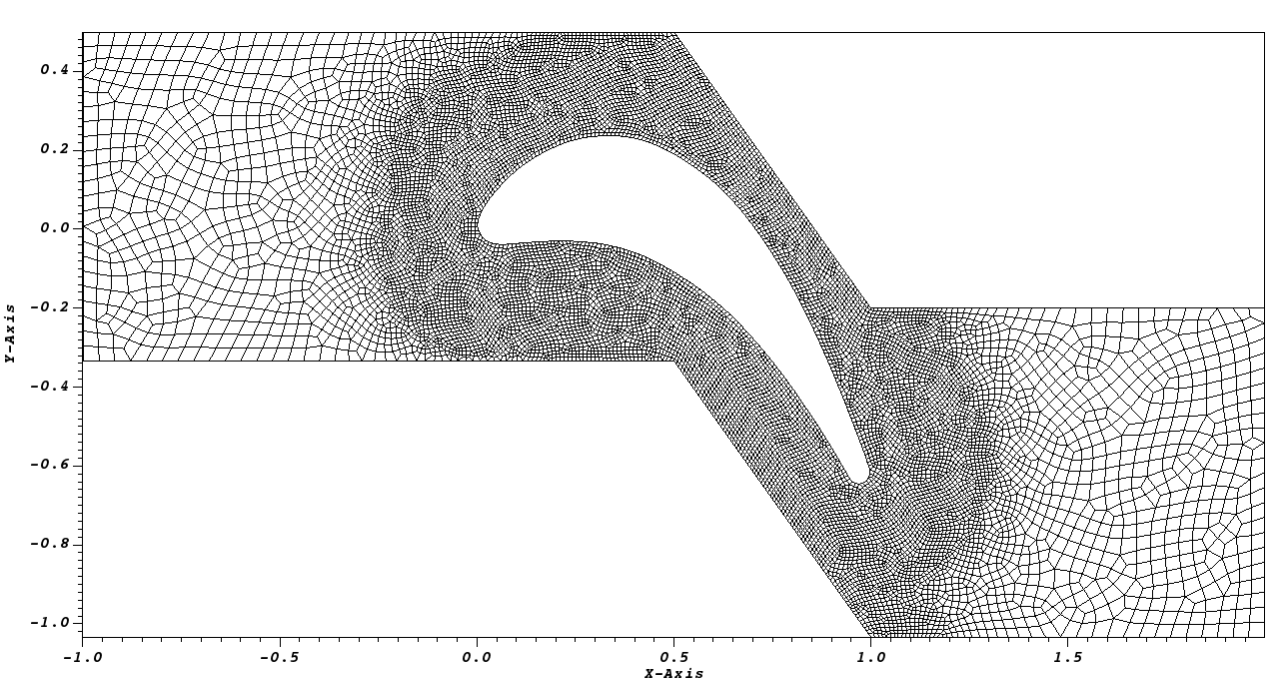
\includegraphics[width=0.88\textwidth]{../Images/fluent_LS59_mesh}
    \caption{Mesh della schiera LS59 realizzata con il software ANSYS Meshing.}
    \label{fig:fluent_ls59_mesh}
\end{figure}

Una volta aperto Fluent si definisce il solutore density-based e si
imposta la pressione di riferimento nulla.
Si attiva l'equazione dell'energia e si seleziona il modello viscoso
Spalart--Allmaras per il caso RANS.
La densità dell'aria segue la legge dei gas perfetti.

Per il caso viscoso il numero di Reynolds è $Re = 554\,140$, da cui si
ricava la viscosità da imporre:
\begin{equation}
    Re = \frac{\rho\, u\, c_x}{\mu\cos\varepsilon}
    \quad\Longrightarrow\quad
    \mu = 4.0819 \times 10^{-4}
    \;\left[\frac{\text{N\,s}}{\text{m}^2}\right]
\end{equation}
Le condizioni al contorno imposte all'inlet sono:
\begin{equation}
    P_0 = 100\,000\ \text{[Pa]},
    \qquad
    T_0 = 300\ \text{[K]},
    \qquad
    \vartheta_{\text{in}} = 30^{\circ}
\end{equation}
dove $\vartheta_{\text{in}}$ è l'angolo del flusso in ingresso rispetto
alla normale al bordo di inlet.
Essendo il campo all'outlet subsonico è necessario imporre anche una
condizione su quel bordo; si impone la pressione statica corrispondente
a un numero di Mach isentropico di uscita pari a $M_{\text{out}} = 1.2$:
\begin{equation}
    P_{\text{outlet}} = 41\,237.7\ \text{[Pa]}
\end{equation}
Il numero di Courant è pari a~5 e si eseguono fino a $10\,000$ iterazioni
per raggiungere la convergenza.

\subsection{\texorpdfstring{$y^+$ sulla superficie della paletta}{y+ sulla superficie della paletta}}

Per risolvere accuratamente lo strato limite è necessario che la mesh sia
tale da garantire $y^+ \leq 5$, in modo che il baricentro della prima
cella di calcolo si trovi all'interno del sottostrato viscoso.
Si riporta in figura~\ref{fig:fluent_ls59_yplus} la distribuzione di
$y^+$ lungo la parete della paletta.

\begin{figure}[H]
    \centering
    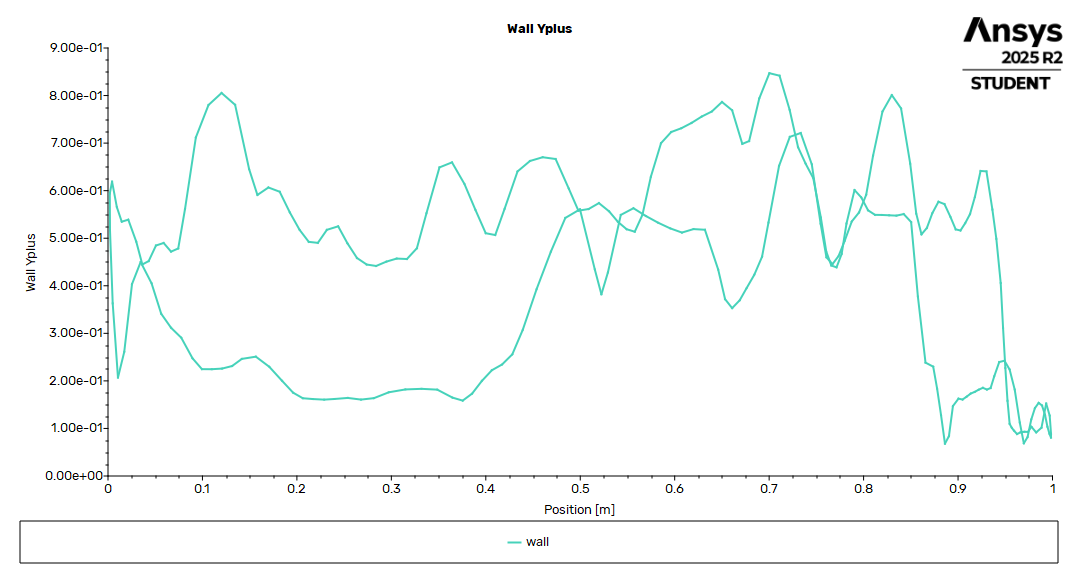
\includegraphics[width=0.78\textwidth]{../Images/fluent_LS59_y+}
    \caption{Distribuzione di $y^+$ lungo la parete della paletta LS59.}
    \label{fig:fluent_ls59_yplus}
\end{figure}

Dal grafico si osserva che in tutte le posizioni $y^+$ è al di sotto della
soglia di~5, confermando che lo strato limite è accuratamente risolto dalla
mesh adottata.

\subsection{Campi di Mach e pressione per caso RANS Fluent}

% ----------------------------------------------------------------
% TODO: immagini non ancora disponibili.
%       Aggiungere:
%         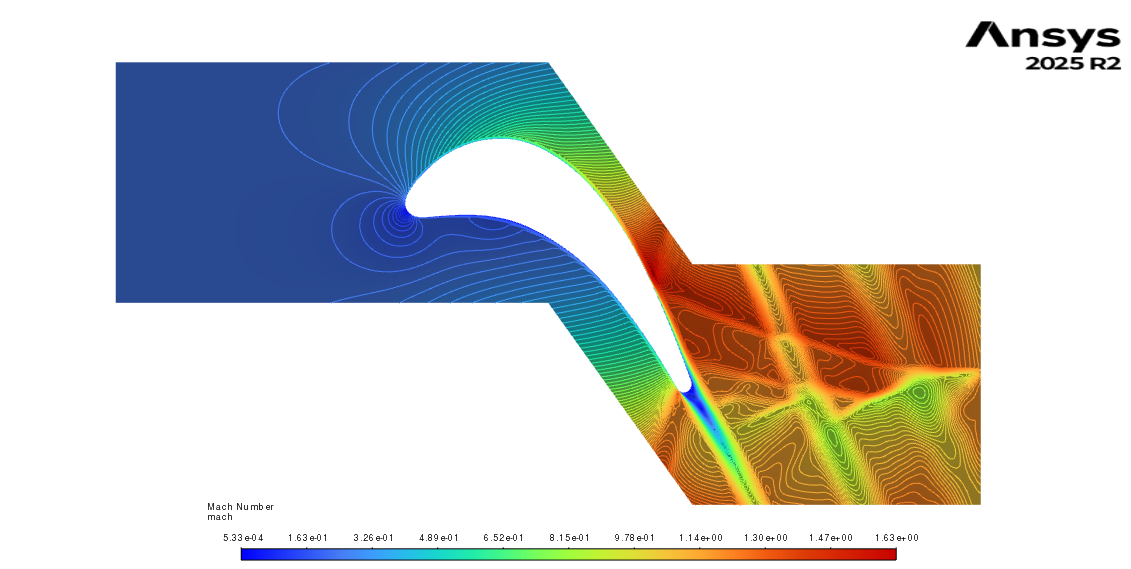
\includegraphics[...]{../Images/fluent_LS59_mach}
%         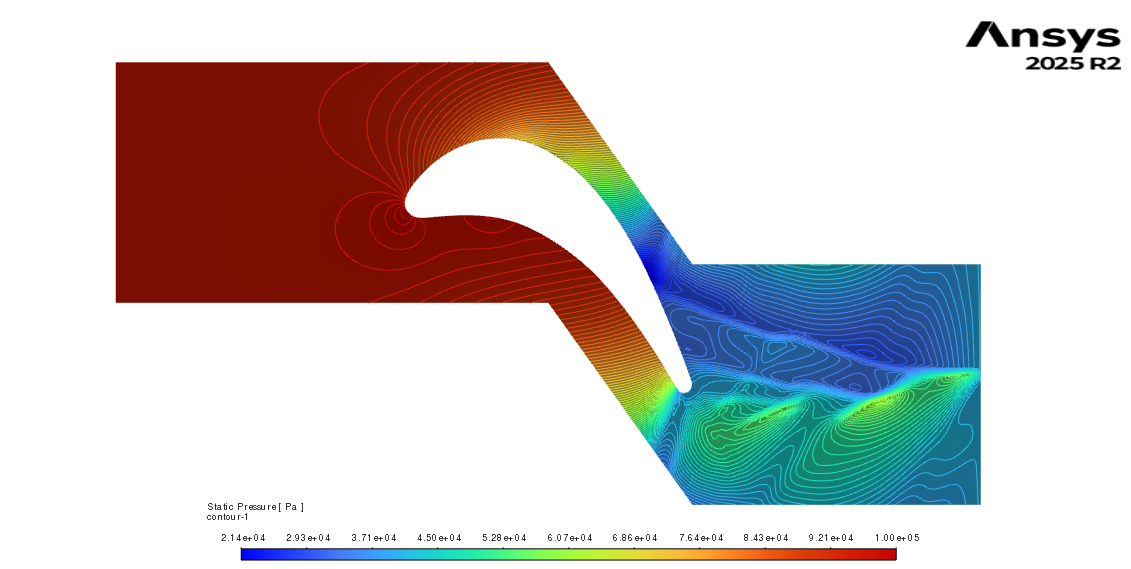
\includegraphics[...]{../Images/fluent_LS59_pressione}
%       quando i file saranno prodotti.
% ----------------------------------------------------------------

I risultati della simulazione RANS vengono visualizzati tramite isolivelli
del numero di Mach e della pressione statica sul dominio di calcolo.
Dall'isolivello del numero di Mach è possibile apprezzare la presenza dello
strato limite sulla superficie della paletta, che porta $M$ ad essere nullo
a parete avendo posizionato il baricentro della prima cella all'interno del
sottostrato viscoso.
Confrontando il caso inviscido con quello RANS si osserva che gli andamenti
delle soluzioni sono pressoché identici: ciò è dovuto al fatto che, in
assenza di separazioni, le equazioni di Eulero colgono bene le distribuzioni
di pressione a parete, le quali nel caso viscoso differiscono solo per la
presenza dello strato limite, che per alti numeri di Reynolds risulta
piccolo rispetto alle dimensioni del profilo.
I valori di pressione ottenuti devono essere normalizzati rispetto alla
pressione totale in ingresso per essere confrontabili con i dati
sperimentali e con i risultati del codice CFD.

\subsection{Profili di strato limite}

% ----------------------------------------------------------------
% TODO: immagini non ancora disponibili.
%       Aggiungere:
%         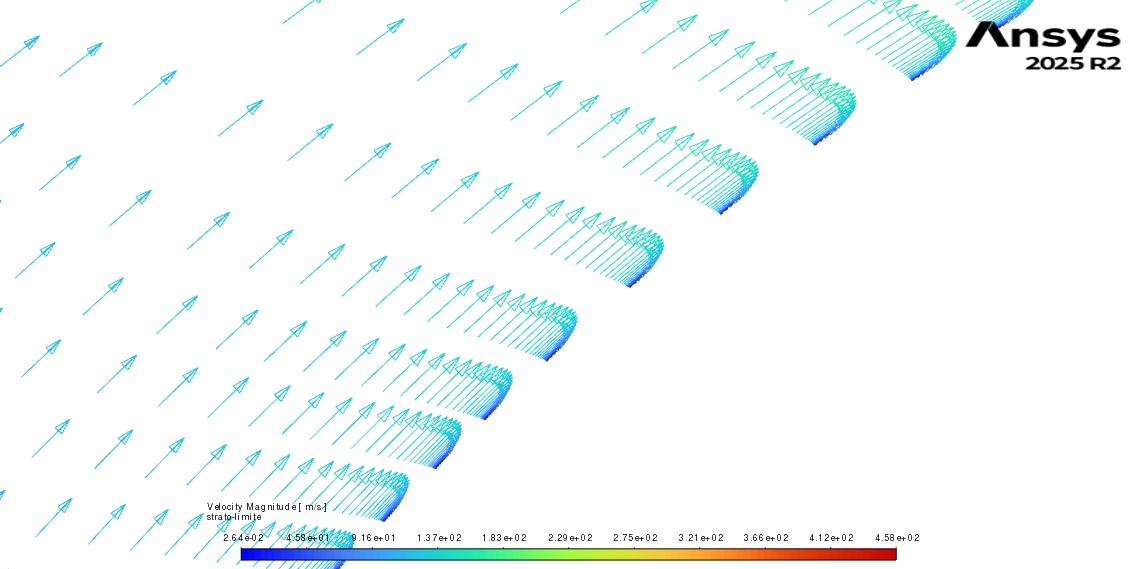
\includegraphics[...]{../Images/fluent_LS59_stratolimite}
%       quando il file sarà prodotto.
% ----------------------------------------------------------------

\subsection{Confronto \texorpdfstring{$M_{is}$}{Mis} a parete: sperimentale vs RANS Fluent vs Eulero Fortran}

% ----------------------------------------------------------------
% TODO: grafico di confronto non ancora disponibile.
%       Sarà fornito dal docente (nota: ``lo daremo dal Penna'').
% ----------------------------------------------------------------

Il grafico di confronto mette in relazione l'andamento del numero di Mach
isentropico a parete $M_{is}$ ricavato sperimentalmente con i risultati
ottenuti dalla simulazione RANS in Fluent e dal codice Eulero sviluppato
in Fortran.
Come discusso in precedenza, tutti i modelli si comportano all'incirca allo
stesso modo nel cogliere i dati sperimentali; le differenze si localizzano
principalmente nel tratto finale del profilo, in prossimità del bordo di
fuga, dove la presenza di spigoli e la generazione di entropia numerica
portano a discrepanze tra i diversi approcci.
L'adozione del modello RANS consente di ottenere risultati più accurati
avendo rilassato l'ipotesi di flusso non viscoso e introdotto la turbolenza.
Si ricorda che i calcoli CFD sono affetti da due tipologie di errori: l'errore
di discretizzazione, controllabile con una griglia più fitta al costo di
maggiore potenza di calcolo, e l'errore di modello, che non può essere
ridotto senza sostituire il modello fisico adottato con uno più raffinato.


% ============================================================
\section{Presa a doppia rampa}
% ============================================================

\subsection{Realizzazione della mesh}

Analogamente al caso LS59, la geometria della presa a doppia rampa viene
importata direttamente come file \texttt{.step} da Gmsh.
Il fattore di scala di~1000 è applicato tramite
\textit{Create} $\to$ \textit{Body Transformation} $\to$ \textit{Scale}.

La mesh è non strutturata con elementi quadrangolari dominanti, con
raffinamento sulla parete inferiore tramite strati di inflazione per
cogliere lo strato limite.
Il raffinamento è applicato solo alla parete inferiore: lo strato limite
si forma anche sulla parete superiore all'interno del condotto, tuttavia
un raffinamento in quella zona introdurrebbe complicazioni legate alla
presenza di uno spigolo, la cui gestione esula dagli obiettivi del presente
lavoro.
La mesh ha le seguenti proprietà:
\begin{itemize}
    \item \textit{Method}: Quadrilateral Dominant
    \item \textit{Element size} (body): $0.01$
    \item \textit{Inflation boundary}: pareti orizzontali
    \item \textit{Inflation type}: Smooth Transition
    \item \textit{First layer height}: $0.272$,
          \textit{Max layers}: $10$,
          \textit{Growth rate}: $1.2$
\end{itemize}
Alle superfici sono stati assegnati i seguenti \textit{named selections}:
\texttt{inlet}, \texttt{outlet}, \texttt{far\_field},
\texttt{lower\_wall}, \texttt{upper\_wall}.

\begin{figure}[H]
    \centering
    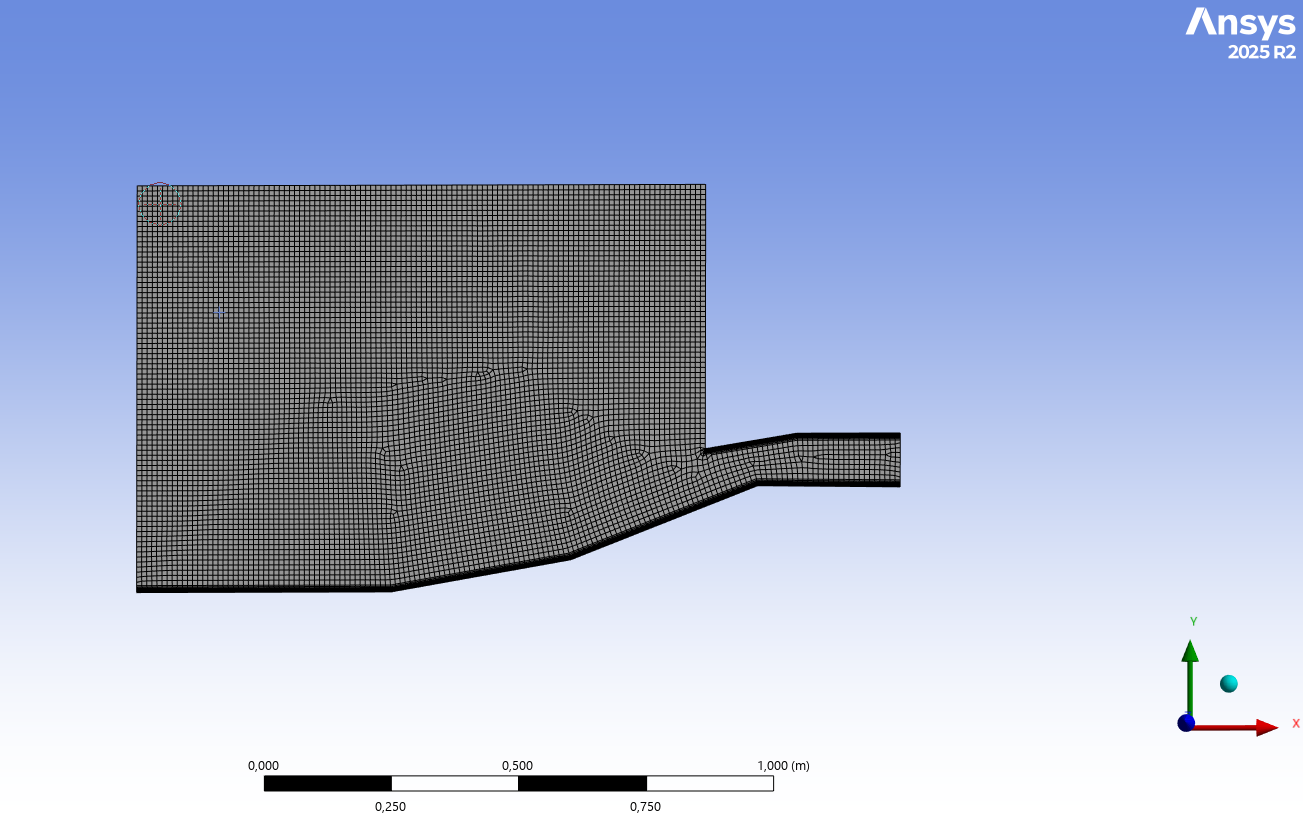
\includegraphics[width=0.88\textwidth]{../Images/fluent_doppiarampa_mesh}
    \caption{Mesh della presa a doppia rampa realizzata con il software ANSYS Meshing.}
    \label{fig:fluent_doppia_mesh}
\end{figure}

Una volta avviato Fluent si seleziona il solutore density-based e si
pone la pressione di riferimento nulla.
Si attiva l'equazione dell'energia, si seleziona il modello di turbolenza
Spalart--Allmaras e si impone la legge dei gas perfetti per la densità.
Il metodo di soluzione è implicito con schema di Roe, discretizzazione
spaziale al secondo ordine upwind con correzione \textit{warped-face};
l'inizializzazione è di tipo ibrido (\textit{Hybrid Initialization}) e
il numero di iterazioni massimo è $1000$.

Il flusso in ingresso è supersonico con $M = 3$; la direzione è normale
al bordo di inlet.
Le condizioni all'inlet sono pressione totale e pressione statica
(ricavata dalla relazione isentropica con $M = 3$) e temperatura totale:
\begin{equation}
    P_0 = 100\,000\ \text{[Pa]},
    \qquad
    P_{\text{in}} = 2722.37\ \text{[Pa]},
    \qquad
    T_0 = 300\ \text{[K]}
\end{equation}
Poiché il campo all'outlet è supersonico non è necessario imporre alcuna
condizione su quel bordo.
Per il caso viscoso il numero di Reynolds è $Re = 1.3\times10^6$, da cui:
\begin{equation}
    Re = \frac{\rho\, u\, L}{\mu}
    \quad\Longrightarrow\quad
    \mu = 1.4946 \times 10^{-5}
    \;\left[\frac{\text{N\,s}}{\text{m}^2}\right]
\end{equation}
L'andamento dei residui può presentare oscillazioni che, secondo quanto
indicato dal docente, non costituiscono un problema per la convergenza
della soluzione.
I risultati vengono visualizzati tramite
\textit{Results} $\to$ \textit{Contour} $\to$ \textit{Static Pressure}
e \textit{Mach Number}, con l'opzione \textit{no global range} per
ottenere isolivelli adattati al campo locale.
Il profilo di pressione a parete è esportato tramite
\textit{Results} $\to$ \textit{Plots} $\to$ \textit{XY Plot},
impostando $y = p(\text{wall})$, $x = \text{direction vector}$,
item \texttt{lower\_wall}, e scrivendo i dati su file.

\subsection{\texorpdfstring{$y^+$ sulla superficie della parete inferiore}{y+ sulla superficie della parete inferiore}}

Si riporta in figura~\ref{fig:fluent_doppia_yplus} la distribuzione di
$y^+$ lungo la parete inferiore della presa a doppia rampa.

\begin{figure}[H]
    \centering
    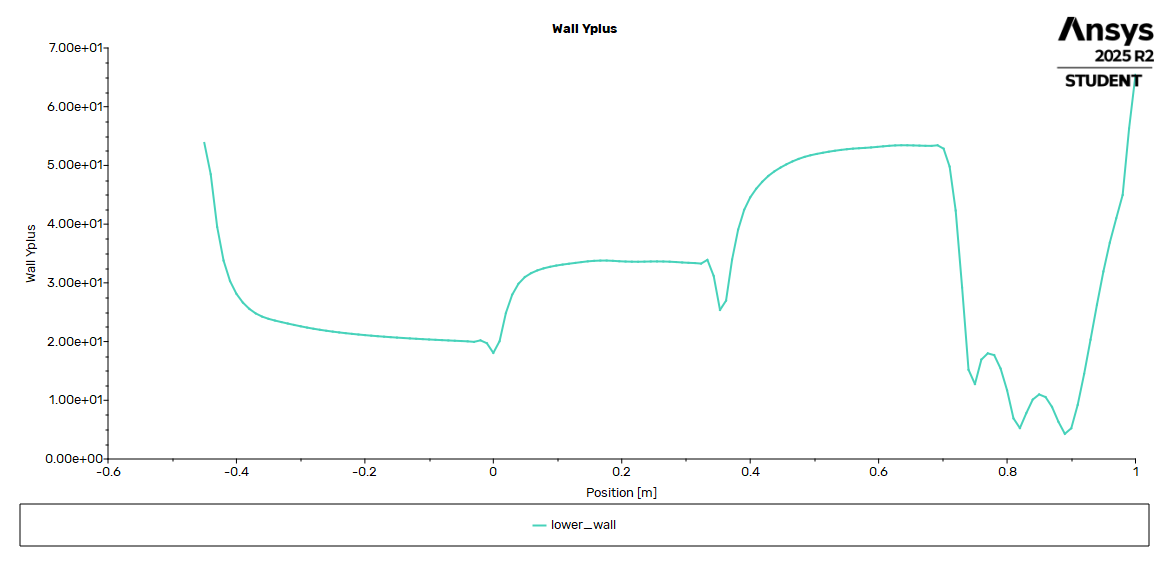
\includegraphics[width=0.78\textwidth]{../Images/fluent_doppiarampa_y+}
    \caption{Distribuzione di $y^+$ lungo la parete inferiore della presa
    a doppia rampa.}
    \label{fig:fluent_doppia_yplus}
\end{figure}

Dal grafico si osserva che nella maggior parte della parete $y^+$ è al di
sopra della soglia di~5, tranne che per una porzione interna della rampa.
Per garantire una corretta risoluzione dello strato limite sull'intera
parete sarebbe necessario ripetere la simulazione aumentando il numero di
layers di inflazione.

\subsection{Campi di Mach e pressione per caso RANS Fluent}

\begin{figure}[H]
    \centering
    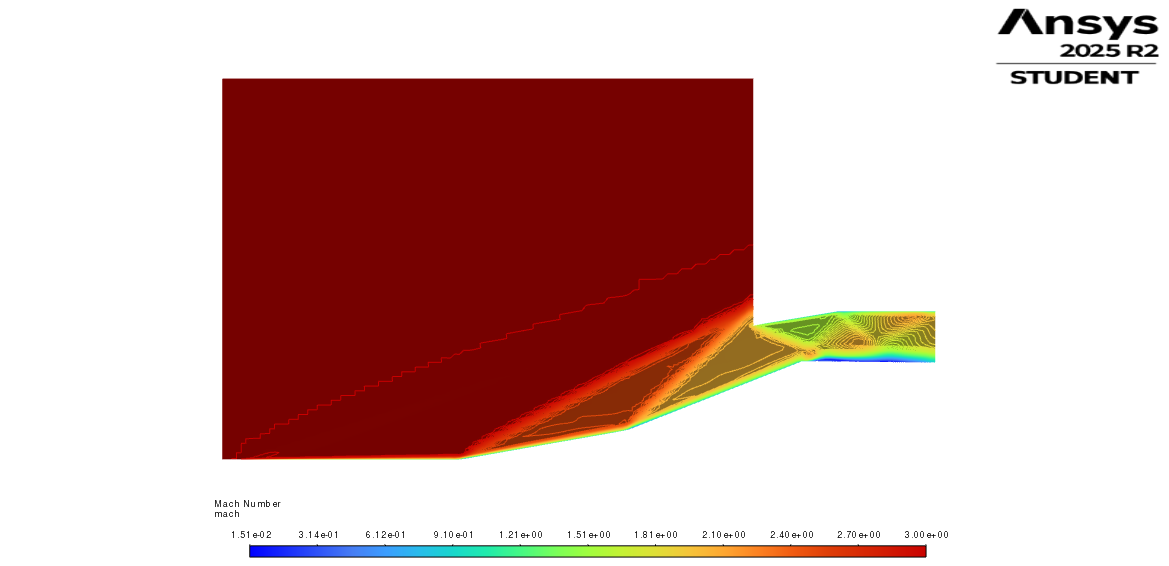
\includegraphics[width=0.88\textwidth]{../Images/fluent_doppiarampa_mach}
    \caption{Isolivelli del numero di Mach -- caso RANS Fluent, presa a doppia
    rampa.}
    \label{fig:fluent_doppia_mach}
\end{figure}

\begin{figure}[H]
    \centering
    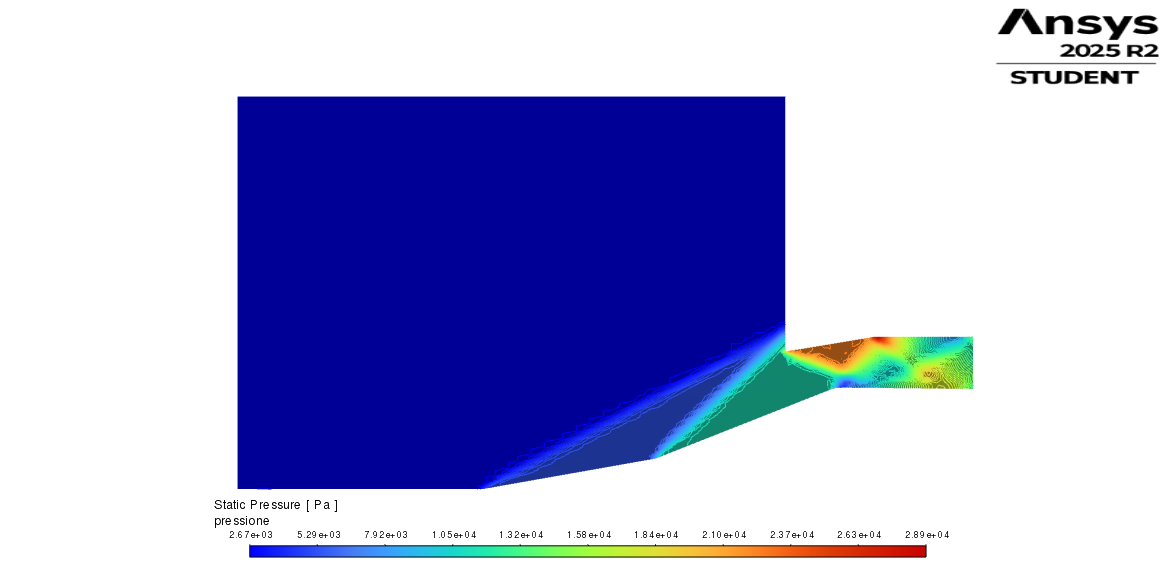
\includegraphics[width=0.88\textwidth]{../Images/fluent_doppiarampa_pressione}
    \caption{Isolivelli di pressione statica -- caso RANS Fluent, presa a doppia
    rampa.}
    \label{fig:fluent_doppia_pressione}
\end{figure}

Nella figura~\ref{fig:fluent_doppia_mach} si apprezza la presenza dello
strato limite che porta il numero di Mach quasi a zero a parete.
Per averlo rigorosamente nullo sarebbe necessario che il baricentro della
prima cella si trovasse all'interno del sottostrato viscoso, condizione
che richiede $y^+ \leq 5$ su tutta la parete.

Un aspetto caratteristico del caso viscoso rispetto a quello inviscido è
la capacità del modello RANS di cogliere la separazione che si genera
all'interno della presa, visibile come bolla di ricircolo in
figura~\ref{fig:fluent_doppia_bolla}.
Tale fenomeno non può essere catturato dal codice Eulero inviscido, che
per definizione non risolve gli effetti viscosi.

\begin{figure}[H]
    \centering
    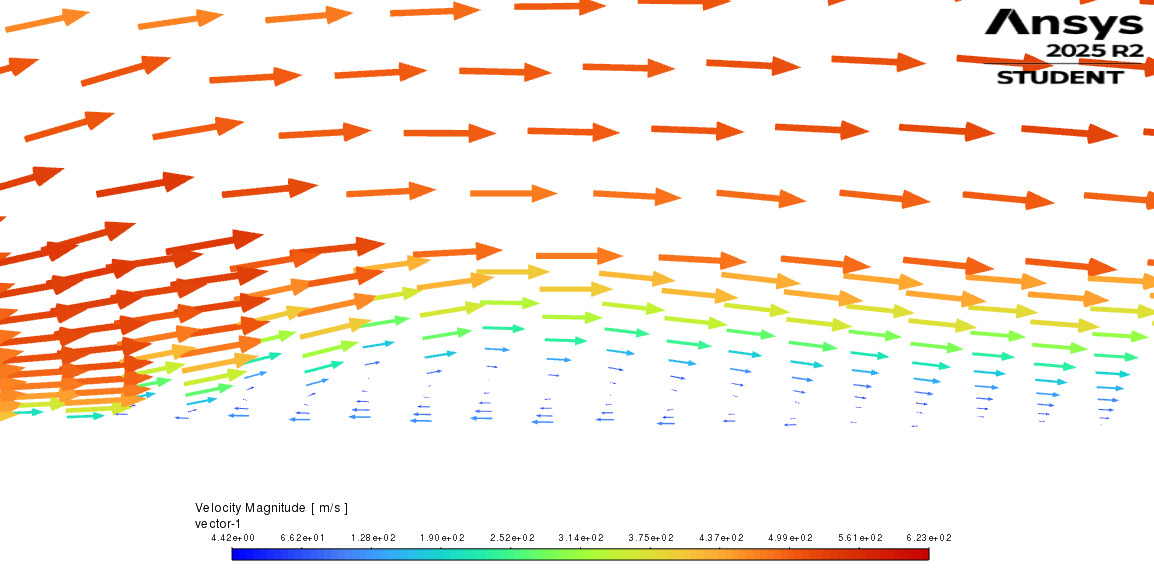
\includegraphics[width=0.78\textwidth]{../Images/fluent_doppiarampa_bollaricircolo}
    \caption{Bolla di ricircolo all'interno della presa a doppia rampa --
    caso RANS Fluent.}
    \label{fig:fluent_doppia_bolla}
\end{figure}

\subsection{Profili di strato limite}

\begin{figure}[H]
    \centering
    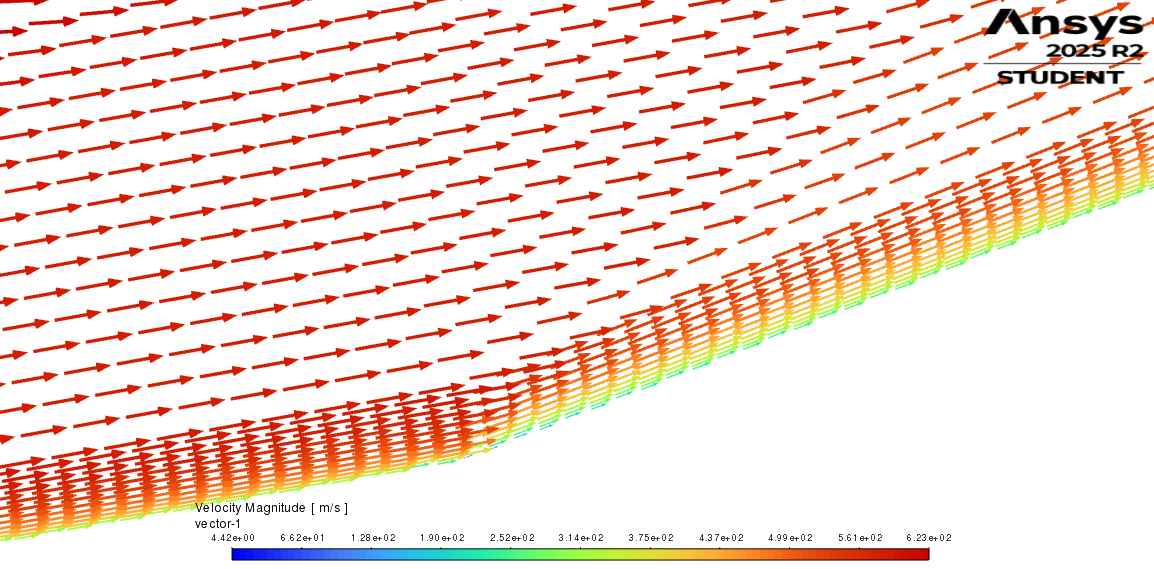
\includegraphics[width=0.78\textwidth]{../Images/fluent_doppiarampa_stratolimite}
    \caption{Profili di strato limite lungo la parete inferiore della presa
    a doppia rampa -- caso RANS Fluent.}
    \label{fig:fluent_doppia_bl}
\end{figure}

\subsection{Confronto \texorpdfstring{$p_w/p^{\circ}$}{pw/p0} sperimentale vs RANS Fluent vs Eulero Fortran}

% ----------------------------------------------------------------
% TODO: grafico di confronto non ancora disponibile.
% ----------------------------------------------------------------

Il grafico di confronto mette a confronto il profilo di pressione a parete
normalizzata $p_w/p^{\circ}$ ricavato sperimentalmente con i risultati
ottenuti dal codice Eulero Fortran e dalla simulazione RANS in Fluent.
I valori di pressione ottenuti da Fluent devono essere normalizzati
rispetto alla pressione totale in ingresso $p^{\circ} = 100\,000$~Pa
per essere confrontabili con i dati sperimentali e con i risultati CFD.

Come si osserva nel grafico, i casi inviscidi (codice Eulero Fortran e
Fluent inviscido) trovano riscontro diretto l'uno con l'altro, mentre
il caso viscoso si comporta differentemente nel tratto finale del dominio.
In assenza di dati sperimentali in quel tratto non è possibile stabilire
quale modello si comporti più correttamente; tuttavia il modello RANS
introduce equazioni aggiuntive e rilassa alcune delle ipotesi del modello
inviscido, per cui ci si aspetta che sia più rappresentativo della fisica
reale, in particolare nelle zone di separazione.
Si ricorda che i calcoli CFD sono affetti da due tipologie di errori:
l'errore di discretizzazione, riducibile con una griglia più fitta al
costo di maggiore potenza di calcolo, e l'errore di modello, che non può
essere controllato senza cambiare il modello fisico adottato con uno più
raffinato.
